

\documentclass{article}
\usepackage{tikz}
\usetikzlibrary{arrows,shapes}
 
\begin{document}
 
 
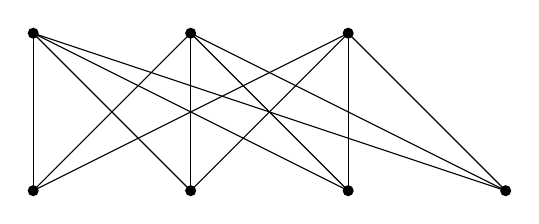
\begin{tikzpicture}[scale=2]
 
   \foreach \i in {1,...,4}
   {
      \path (\i,0) coordinate (X\i);
      \fill (X\i) circle (1pt);
   }
 
   \foreach \j in {1,...,3}
   {
      \path (\j,1) coordinate (Y\j);
      \fill (Y\j) circle (1pt);
   }
 
   \foreach \i in {1,...,4}
   {
      \foreach \j in {1,...,3}
      {
         \draw (X\i) -- (Y\j);
      }
   }
\end{tikzpicture}

\end{document}

